\section{2020 年 12 月 12 日答疑记录}

\subsection{弧度制}

角的大小用来描述角的两边 (始边和终边) 张开的幅度. 度量角的大小的方法中, 常见的为如下两种:

(1) 将射线绕定点旋转一周所形成的角 (称为周角) 等分为 $360$~份, 每一份的大小记为 $1^\circ$. 所以周角的大小是 $360^\circ$, 并这种方法称为角度制. 

(2) 将角的顶点放在圆心, 利用所截弧长来定义角的大小. 当圆心角固定时, 若半径越大, 则所对弧长也越大, 所以定义弧长与半径的比例为圆心角的大小, 并称这种方法为弧度制. 此时周角的大小是 $\dfrac{2\pi r}r= 2\pi\,\mathrm{rad}$. $\mathrm{rad}$ 是弧度制的单位, 念作 ``弧度'' (radian), 通常略去不写.

根据相似形对应线段或弧成比例, 对固定的圆心角, 弧长与半径的比例为定值, 所以第二种方法是合理的. 

    \begin{center}
        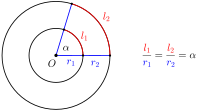
\includegraphics[scale=1]{2020-1218-1940-crop}
    \end{center}
    
高中数学更常用的是弧度制. 由定义, $360^\circ =2\pi$, 并应熟记特殊角 $0^\circ$, $30^\circ$, $45^\circ$, $60^\circ$, $90^\circ$, $120^\circ$, $135^\circ$, $150^\circ$, $180^\circ$ 的角度和弧度.

    \begin{center}
        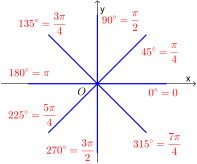
\includegraphics[scale=1]{2020-1220-0920-crop}\quad
        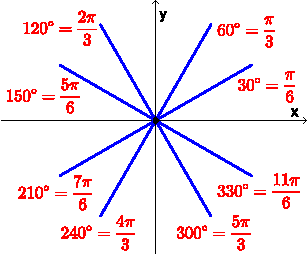
\includegraphics[scale=1]{2020-1220-0930-crop}
    \end{center}
    
容易得到弧度与角度互换公式: 
\[1\,\mathrm{rad}= \Big(\frac{180}{\pi}\Big)^{\circ} \approx 57.3^{\circ}, \quad
    1^{\circ}= \frac{\pi}{180}\,\mathrm{rad}.\]
若圆心角 $\alpha$ (弧度制, 可能为负) 所对的弧长为 $l$, 则 $|\alpha|=\dfrac{l}{r}$, 其中 $r$ 是圆的半径. 此外还有弧长公式 $l=|\alpha|r$, 和扇形面积公式
\[S= \dfrac{1}{2}lr= \dfrac{1}{2}|\alpha| r^2\quad 
    \text{(类似于三角形面积公式)}.\]

\begin{example}
    求终边落在直线 $y=-x$ 上的角 $\alpha$ 的集合.
\end{example}
\begin{solution}
    直线 $y=-x$ 为第二、四象限的角平分线, 作图易知, 所求集合为
    \[\{\alpha\mid\ 135^\circ+k\cdot 180^\circ\}
        = \biggl\{\alpha\biggm| \frac{3\pi}4+k\pi\biggr\}.\]
    以上两个集合, 只写其中一个即可 (用弧度制相对来说更简洁).
\end{solution}

\begin{example}\label{exa:201220-1030}
    已知某扇形的半径为 $10$, 面积为 $\dfrac{50\pi}3$, 求该扇形的圆心角大小.
\end{example}
\begin{solution}
    设该扇形的圆心角弧度大小为 $\alpha$, 半径为 $r$, 则其面积 \[S=\frac12\alpha r^2,\quad\text{即}\quad 
        \frac{50\pi}3= \frac12 \alpha\cdot 10^2.\]
    解得 $\alpha=\dfrac\pi3$.
\end{solution}
\begin{remark}
    例~\ref{exa:201220-1030} 也可以用角度制来解: 设该扇形的圆心角角度大小为 $\alpha$, 半径为 $r$, 则其面积 $S=\dfrac{\alpha}{360^\circ} \pi r^2$, 可求得 $\alpha=60^\circ$. 用角度制计算相对更简单一些.
\end{remark}

\subsection{任意角三角函数的定义}

  如下方左图, 设 $\alpha$ 是任意一个角, 顶点为坐标原点, 
  始边为 $x$~正半轴, $P(x, y)$ 是终边上任意一点 (异于原点), 
  它与原点的距离是 $r= \sqrt{x^2+ y^2}> 0$, 那么 
  \[\sin\alpha= \frac{y}{r},\quad
    \cos\alpha= \frac{x}{r},\quad 
    \tan\alpha= \frac{y}{x}\ (x\neq 0).\]
  三角函数值只与角的大小有关, 而与终边上点~$P$ 的位置无关. 由定义容易判断各象限内的角的三角函数值的正负号. 若点~$P$ 恰在单位圆 (圆心为原点且半径为 $1$) 上, 取点~$A(1,0)$, 并作 $PM\perp OA$ 于点 $M$, 作 $TA\perp OA$ 并交射线~$OP$ 于点~$T$, 则此时 $r=1$, 且 (类似锐角三角函数的定义)
  \[\sin\alpha= y,\quad
    \cos\alpha= x,\quad 
    \tan\alpha= \frac{AT}{OA}= AT\ (x\neq 0).\]
  对 $\angle{POA}$ 来说, $MP$ 为正弦线, $OM$ 为余弦线, $AT$ 为正切线, 
  且各线段均为有向线段 (即规定了正方向, 所以表示时带正负号). 常用的三角函数值, 参考下方右图. 由此可以写出其他特殊角 ($120^\circ$, $135^\circ$, $150^\circ$ 等) 的各三角函数值, 如 $\sin 120^\circ= \dfrac{\sqrt3}2$, $\cos135^\circ= -\dfrac{\sqrt2}2$.
  
  \begin{small}
    \begin{minipage}[t]{0.35\linewidth}
    \centering
    \begin{tikzpicture}[scale=1.1]
      \draw[-{Stealth[scale=0.8]}] (-1.2,0) -- (1.4,0) node[below] {$x$};
      \draw[-{Stealth[scale=0.8]}] (0,-1.2) -- (0,1.3) node[left] {$y$};
      \draw (0,0) circle (1) node[anchor=45] {$O$} coordinate (O);
      \def\myangle{40};
      \pgfmathparse{tan(\myangle)};
      \coordinate (B) at (\myangle:1.6);
      \draw[fill=black] (1,0) circle (0.6pt) coordinate (A)
        +(0.1,0) node[below] {$A$};
      \draw[fill=black] (1,\pgfmathresult) coordinate (T) circle (0.6pt) 
        node[above] {$T$} ;
      \draw[fill=black] (\myangle:1) circle (0.6pt) coordinate (P)
       +(0,0.06) node[above] {$P$};
      \draw[fill=black] ($(O)!(P)!(A)$) coordinate (M) circle (0.6pt) 
        node[below] {$M$};
      \draw (O)--(B) (M)--(P) (A)--(T);      
    \end{tikzpicture}
    \end{minipage}
    \hskip 1cm%
    \begin{minipage}[t]{0.55\linewidth}
    \centering
    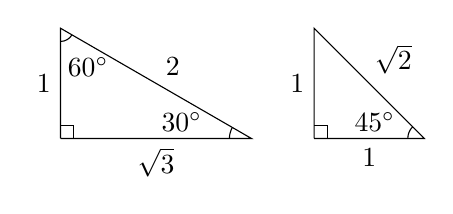
\begin{tikzpicture}[scale=1.4]
      \pgfmathparse{sqrt(3)};
      \draw (0,0) coordinate (A)-- node[below] {$\sqrt3$} 
        (1.732,0) coordinate (B)-- node[anchor=225] {$2$}
        (0,1) coordinate (C)--node[left] {$1$} (0,0);
      \draw (A)++(0,0.12)--++(0.12,0)--++(0,-0.12);
      \draw (C)+(0,-0.12) arc (270:330:0.12);
      \draw (B)+(-0.2,0) arc (180:150:0.2);
      \draw (A)+(0.25,0.65) node {$60^\circ$} +(1.1,0.15) node {$30^\circ$};
      \draw (2.3,0) coordinate (D)-- node[below] {$1$} 
        +(1,0) coordinate (E)-- node[anchor=225] {$\sqrt2$}
        +(0,1) coordinate (F)--node[left] {$1$} (2.3,0);
      \draw (D)++(0,0.12)--++(0.12,0)--++(0,-0.12);
      \draw (E)+(-0.15,0) arc (180:135:0.15);
      \draw (D)+(0.55,0.15) node {$45^\circ$};
    \end{tikzpicture}
    \end{minipage}
    \end{small}

\begin{example}
    $\sin6\underline{\qquad}0$. (填 ``$>$'' 或 ``$<$'')
\end{example}
\begin{solution}
    注意题中的 $6$ 是弧度制, 而 $360^\circ=2\pi\approx 6.28$, 所以 $6$~弧度在第四象限. 由正弦的定义, $\sin 6<0$.
\end{solution}
\begin{remark}
    类似地, $1$~弧度在第一象限, $2$ 弧度和 $3$ 弧度都在第二象限, 所以
    \[\sin 1,\ \sin 2,\ \sin 3>0,\quad 
        \cos 1>0,\quad \cos 2,\ \cos 3<0.\]
    此外, 画图可知 $\sin 1< \sin 2$.
\end{remark}

\begin{example}
    已知角 $\alpha$ 的终边经过点 $P(-x,-12)$, 
    且 $\cos\alpha=-\dfrac5{13}$, 求 $x$ 的值.
\end{example}
\begin{solution}
    由余弦定义, 
    \[\cos\alpha= \frac{-x}{\sqrt{(-x)^2+(-12)^2}}= -\frac5{13},\quad
    \text{解得}\ x=\pm5.\]
    经检验, $x=5$  (或由余弦值为负知点~$P$ 在第二、三象限, 所以 $-x<0$ 即 $x>0$).
\end{solution}